% Options for packages loaded elsewhere
\PassOptionsToPackage{unicode}{hyperref}
\PassOptionsToPackage{hyphens}{url}
\PassOptionsToPackage{dvipsnames,svgnames,x11names}{xcolor}
%
\documentclass[
]{report}

\usepackage{amsmath,amssymb}
\usepackage{iftex}
\ifPDFTeX
  \usepackage[T1]{fontenc}
  \usepackage[utf8]{inputenc}
  \usepackage{textcomp} % provide euro and other symbols
\else % if luatex or xetex
  \usepackage{unicode-math}
  \defaultfontfeatures{Scale=MatchLowercase}
  \defaultfontfeatures[\rmfamily]{Ligatures=TeX,Scale=1}
\fi
\usepackage{lmodern}
\ifPDFTeX\else  
    % xetex/luatex font selection
\fi
% Use upquote if available, for straight quotes in verbatim environments
\IfFileExists{upquote.sty}{\usepackage{upquote}}{}
\IfFileExists{microtype.sty}{% use microtype if available
  \usepackage[]{microtype}
  \UseMicrotypeSet[protrusion]{basicmath} % disable protrusion for tt fonts
}{}
\makeatletter
\@ifundefined{KOMAClassName}{% if non-KOMA class
  \IfFileExists{parskip.sty}{%
    \usepackage{parskip}
  }{% else
    \setlength{\parindent}{0pt}
    \setlength{\parskip}{6pt plus 2pt minus 1pt}}
}{% if KOMA class
  \KOMAoptions{parskip=half}}
\makeatother
\usepackage{xcolor}
\usepackage[top=30mm,left=20mm]{geometry}
\setlength{\emergencystretch}{3em} % prevent overfull lines
\setcounter{secnumdepth}{-\maxdimen} % remove section numbering
% Make \paragraph and \subparagraph free-standing
\ifx\paragraph\undefined\else
  \let\oldparagraph\paragraph
  \renewcommand{\paragraph}[1]{\oldparagraph{#1}\mbox{}}
\fi
\ifx\subparagraph\undefined\else
  \let\oldsubparagraph\subparagraph
  \renewcommand{\subparagraph}[1]{\oldsubparagraph{#1}\mbox{}}
\fi


\providecommand{\tightlist}{%
  \setlength{\itemsep}{0pt}\setlength{\parskip}{0pt}}\usepackage{longtable,booktabs,array}
\usepackage{calc} % for calculating minipage widths
% Correct order of tables after \paragraph or \subparagraph
\usepackage{etoolbox}
\makeatletter
\patchcmd\longtable{\par}{\if@noskipsec\mbox{}\fi\par}{}{}
\makeatother
% Allow footnotes in longtable head/foot
\IfFileExists{footnotehyper.sty}{\usepackage{footnotehyper}}{\usepackage{footnote}}
\makesavenoteenv{longtable}
\usepackage{graphicx}
\makeatletter
\def\maxwidth{\ifdim\Gin@nat@width>\linewidth\linewidth\else\Gin@nat@width\fi}
\def\maxheight{\ifdim\Gin@nat@height>\textheight\textheight\else\Gin@nat@height\fi}
\makeatother
% Scale images if necessary, so that they will not overflow the page
% margins by default, and it is still possible to overwrite the defaults
% using explicit options in \includegraphics[width, height, ...]{}
\setkeys{Gin}{width=\maxwidth,height=\maxheight,keepaspectratio}
% Set default figure placement to htbp
\makeatletter
\def\fps@figure{htbp}
\makeatother

\usepackage{float}
\usepackage{tabularray}
\usepackage[normalem]{ulem}
\usepackage{graphicx}
\UseTblrLibrary{booktabs}
\UseTblrLibrary{siunitx}
\NewTableCommand{\tinytableDefineColor}[3]{\definecolor{#1}{#2}{#3}}
\newcommand{\tinytableTabularrayUnderline}[1]{\underline{#1}}
\newcommand{\tinytableTabularrayStrikeout}[1]{\sout{#1}}
\makeatletter
\makeatother
\makeatletter
\makeatother
\makeatletter
\@ifpackageloaded{caption}{}{\usepackage{caption}}
\AtBeginDocument{%
\ifdefined\contentsname
  \renewcommand*\contentsname{Table of contents}
\else
  \newcommand\contentsname{Table of contents}
\fi
\ifdefined\listfigurename
  \renewcommand*\listfigurename{List of Figures}
\else
  \newcommand\listfigurename{List of Figures}
\fi
\ifdefined\listtablename
  \renewcommand*\listtablename{List of Tables}
\else
  \newcommand\listtablename{List of Tables}
\fi
\ifdefined\figurename
  \renewcommand*\figurename{Figure}
\else
  \newcommand\figurename{Figure}
\fi
\ifdefined\tablename
  \renewcommand*\tablename{Table}
\else
  \newcommand\tablename{Table}
\fi
}
\@ifpackageloaded{float}{}{\usepackage{float}}
\floatstyle{ruled}
\@ifundefined{c@chapter}{\newfloat{codelisting}{h}{lop}}{\newfloat{codelisting}{h}{lop}[chapter]}
\floatname{codelisting}{Listing}
\newcommand*\listoflistings{\listof{codelisting}{List of Listings}}
\makeatother
\makeatletter
\@ifpackageloaded{caption}{}{\usepackage{caption}}
\@ifpackageloaded{subcaption}{}{\usepackage{subcaption}}
\makeatother
\makeatletter
\@ifpackageloaded{tcolorbox}{}{\usepackage[skins,breakable]{tcolorbox}}
\makeatother
\makeatletter
\@ifundefined{shadecolor}{\definecolor{shadecolor}{rgb}{.97, .97, .97}}
\makeatother
\makeatletter
\makeatother
\makeatletter
\makeatother
\ifLuaTeX
  \usepackage{selnolig}  % disable illegal ligatures
\fi
\IfFileExists{bookmark.sty}{\usepackage{bookmark}}{\usepackage{hyperref}}
\IfFileExists{xurl.sty}{\usepackage{xurl}}{} % add URL line breaks if available
\urlstyle{same} % disable monospaced font for URLs
\hypersetup{
  pdftitle={Modelling: 2nd Attempt},
  pdfauthor={Eric},
  colorlinks=true,
  linkcolor={blue},
  filecolor={Maroon},
  citecolor={Blue},
  urlcolor={Blue},
  pdfcreator={LaTeX via pandoc}}

\title{Modelling: 2nd Attempt}
\author{Eric}
\date{}

\begin{document}
\maketitle
\begin{abstract}
The most densely populated areas have the worst energy intensity. Wind
energy generated has a positive relationship with energy intensity,
meaning more wind energy is related to worse energy intensity. Only a
couple months have a siginificant affect on predicting energy intensity.
And different months do not have significant affect mean intensity
overall. Only when combined with CCAA does it show an effect.
\end{abstract}
\ifdefined\Shaded\renewenvironment{Shaded}{\begin{tcolorbox}[enhanced, boxrule=0pt, interior hidden, frame hidden, borderline west={3pt}{0pt}{shadecolor}, breakable, sharp corners]}{\end{tcolorbox}}\fi

\renewcommand*\contentsname{Table of contents}
{
\hypersetup{linkcolor=}
\setcounter{tocdepth}{2}
\tableofcontents
}
\newpage

\textbf{Hypothesis 1:}\\
An increase in wind energy generated is associated with a decrease in
energy intensity, for each CCAA in 2023.

\textbf{Method:} Sectional modelling

\hypertarget{data-wrangling}{%
\section{Data wrangling}\label{data-wrangling}}

\hypertarget{correlations}{%
\section{Correlations}\label{correlations}}

The Pearson's correlation between wind energy generated (MWh) and energy
intensity (MWh/€) is 0.2542. But the correlation changes to 0.6658 when
you use the logged wind generation. That suggests that the relationship
is log-linear. In other words, a multiplicative change to wind energy is
associated with a linear unit of change in energy intensity. Since the
correlation is positive, we can say that a multiplicative increase in
wind energy is associated with a linear increase in energy intensity.

\begin{figure}

{\centering 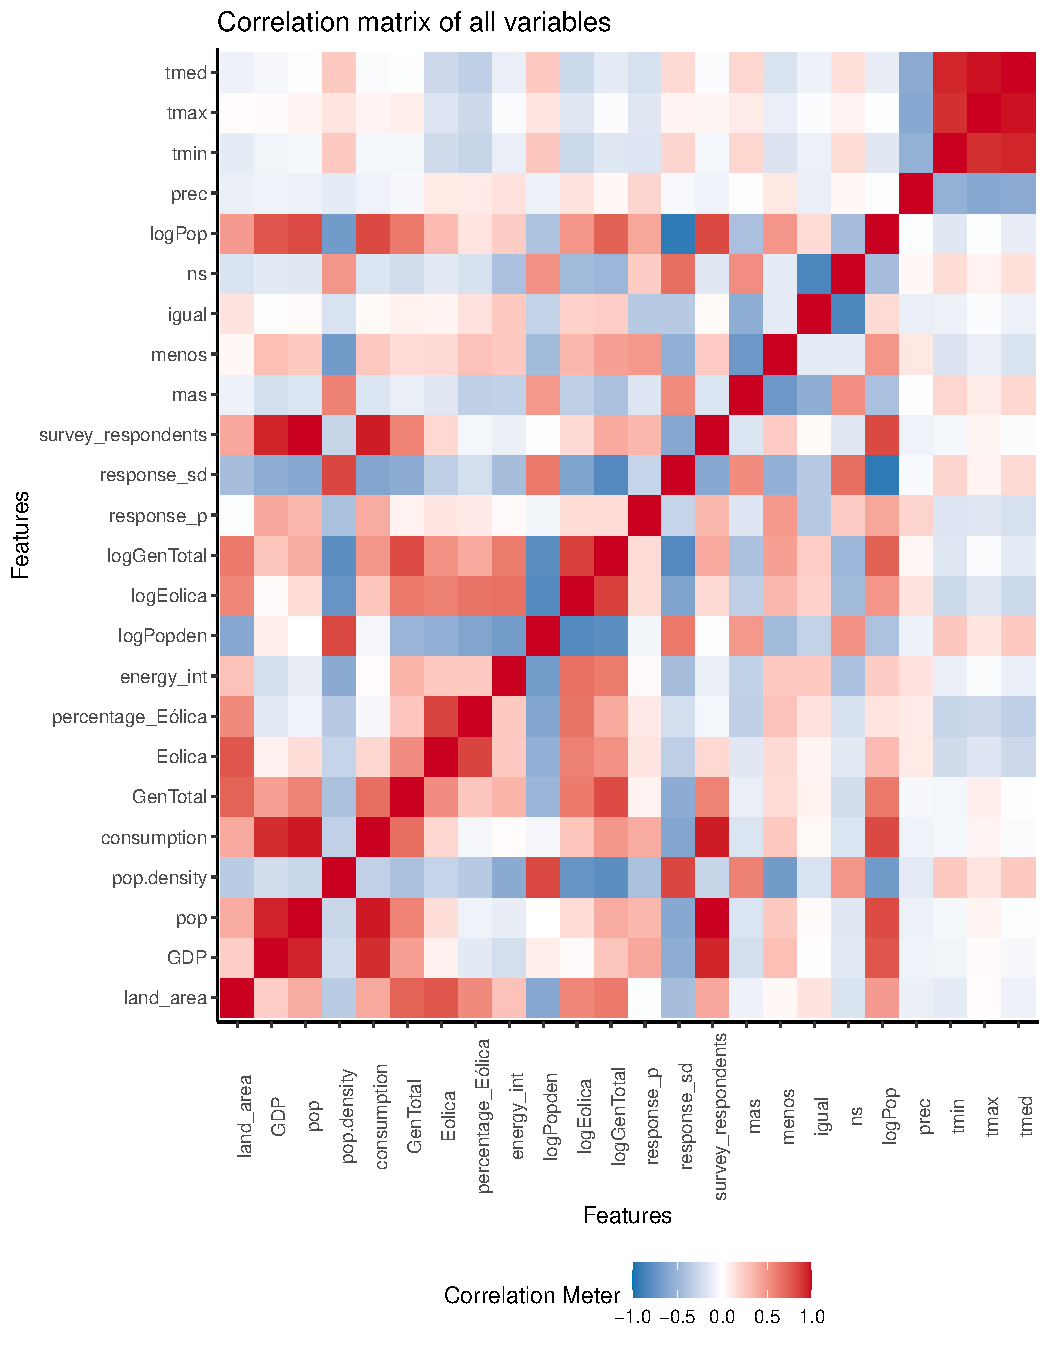
\includegraphics{Modelling_Energy_Intensity-V3_files/figure-pdf/cor-plot-1.pdf}

}

\caption{Correlation Matrix}

\end{figure}

\hypertarget{linear-models}{%
\section{Linear Models}\label{linear-models}}

\texttt{lm\_basic}\strut \\
First, I ran a simple linear regression with \texttt{logEolica} and
\texttt{percentage\_Eólica} as the only predictor variables. The results
suggest that wind energy generation has a relationship with energy
intensity. The logged output of wind energy, \texttt{logEolica}, is
strongly related to energy intensity. The percentage of total
electricity generated in a CCAA, \texttt{percentage\_Eólica}, is not as
strongly related. For two CCAA with the same amount of wind energy
generated, the one with a higher percentage is very likely to have a
lower energy intensity. Furthermore, the Adjusted R\textsuperscript{2}
is almost 50\%, which is good.

\texttt{for\_tune}\strut \\
Next, I ran a forward selection regression, with 10 predictors. I did
not include month or CCAA. The results showed that four predictors is
good, because after that the RMSE increased with five or six variables.
You can see that the best model with six predictors were:
\texttt{logEolica}, \texttt{logPop}, \texttt{mas}, \texttt{logGenTotal},
\texttt{prec}, and \texttt{tmin}. The best model with seven predictors
included the same plus \texttt{ns}. Although the RMSE and
R\textsuperscript{2} keep increasing as you add more predictors, the
first jump is from six to seven. Before that, adding a variable to the
model does not make the overall model's variation metrics improve
significantly. And after seven variables, I am afraid that there would
be very much collinearity.

I was hesitant to include \texttt{ns} because it has a clear outlier due
to low sample size. This variable represents the percent of respondents
who answered ``I don't know'' to the survey question about environmental
degration in 10 years. The problem is that \textbf{Ceuta} had a very low
sample size and then had a much higher proportion of ``I don't know''
answers than the others. I have decided to include it anyway because the
rest of the data looks good.

\hypertarget{picking-the-right-predictors}{%
\subsection{Picking the right
predictors:}\label{picking-the-right-predictors}}

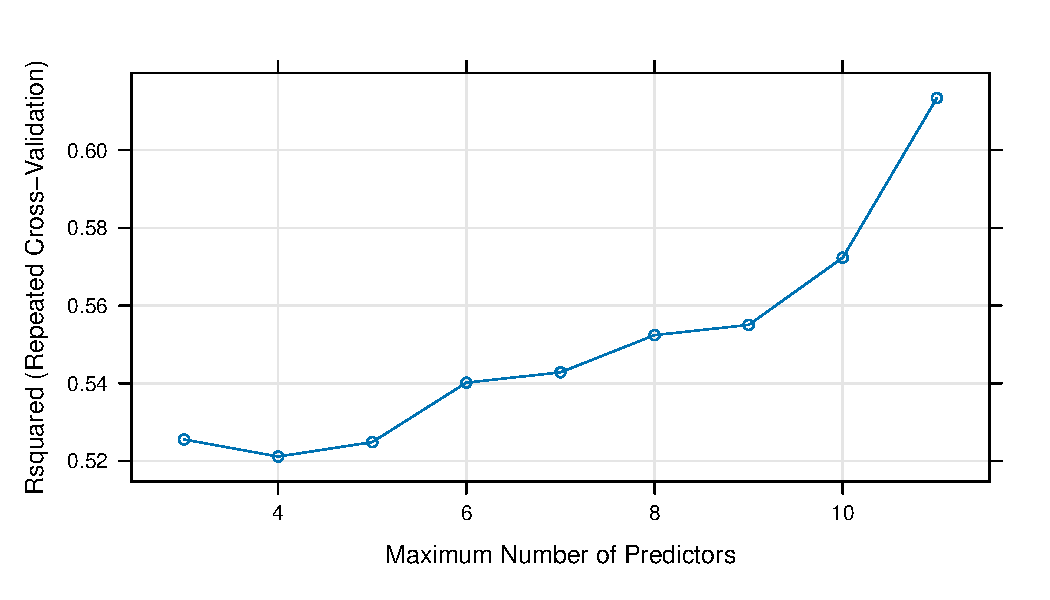
\includegraphics{Modelling_Energy_Intensity-V3_files/figure-pdf/lm-1.pdf}

\begin{verbatim}
(Intercept)   logEolica         mas   logPopden logGenTotal      logPop 
 16.6587012   0.8335747  -0.3320435  -1.1979871   2.4832510  -1.6979768 
       prec 
  0.3256555 
\end{verbatim}

\begin{verbatim}
(Intercept)   logEolica  response_p         mas   logPopden logGenTotal 
 16.6587012   0.7728670   0.1400357  -0.3239923  -1.2084357   2.5846922 
     logPop        prec 
 -1.8019825   0.2998461 
\end{verbatim}

\hypertarget{is-month-a-significant-predictor}{%
\subsection{\texorpdfstring{Is \texttt{month} a significant
predictor?}{Is month a significant predictor?}}\label{is-month-a-significant-predictor}}

\texttt{aov\_month}\strut \\
I ran several ANOVA models to test if month has a strong relationship
with energy intensity, using wind energy and CCAA as covariates.\\
\emph{Null Hypothesis:} There is no difference in mean energy intensity
across months.\\
\emph{Alternate Hypothesis:} At least one month has a mean significantly
different from the others.

\[
H_0: \mu_{Jan} = \mu_{Feb} = \mu_{Mar} =  ...  = \mu_{Dec} 
\]

For the first ANOVA model, I only included \texttt{month}, which did not
return statistically significant results. Here we cannot reject the null
hypothesis that different months have different mean energy intensity
across Spain.

The second ANOVA model includes logged wind energy generated as a
covariate and an interaction term with \texttt{month}. The
\texttt{logEolica} covariate is significant
(\texttt{p-value\ \textless{}\ 2e-16}) but neither of the terms with
month are significant. This means that given the wind energy generated,
the different months do not have a statistically significant effect on
energy intensity.

The third ANOVA model includes autonomous community \texttt{CCAAnombre}

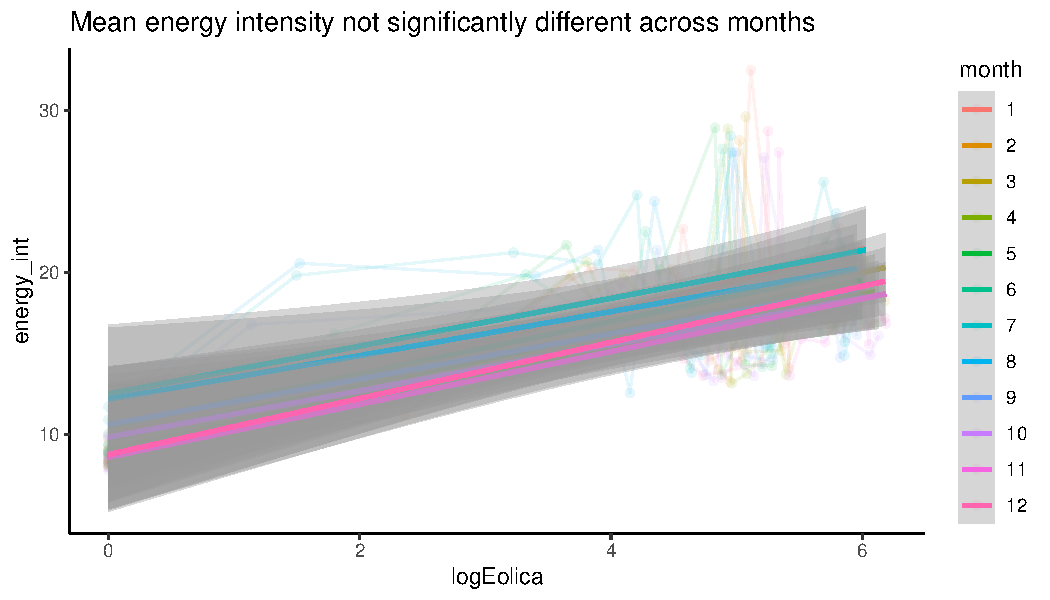
\includegraphics{Modelling_Energy_Intensity-V3_files/figure-pdf/aov-1.pdf}

\hypertarget{ccaa-is-a-significant-predictors}{%
\subsection{CCAA is a significant
predictors}\label{ccaa-is-a-significant-predictors}}

Although CCAA seems to be a better predictor than month, the best model
includes \texttt{month\ +\ CCAAnombre}. Having CCAA by itself won't do
as well as including month, but it is still very good, as you can see in
the RSS value compared to the other models.

\begin{verbatim}
Analysis of Variance Table

Model 1: energy_int ~ month
Model 2: energy_int ~ month * logEolica
Model 3: energy_int ~ month * percentage_Eólica
Model 4: energy_int ~ month + CCAAnombre
Model 5: energy_int ~ CCAAnombre
  Res.Df    RSS  Df Sum of Sq       F    Pr(>F)    
1    216 5245.2                                    
2    204 2791.9  12    2453.3 143.204 < 2.2e-16 ***
3    204 4803.3   0   -2011.4                      
4    198  282.7   6    4520.6 527.745 < 2.2e-16 ***
5    209  480.1 -11    -197.4  12.569 < 2.2e-16 ***
---
Signif. codes:  0 '***' 0.001 '**' 0.01 '*' 0.05 '.' 0.1 ' ' 1
\end{verbatim}

\hypertarget{mixed-models-with-ccaa-as-random-effect}{%
\subsection{Mixed models with CCAA as Random
Effect}\label{mixed-models-with-ccaa-as-random-effect}}

\texttt{lmer\_basic}\strut \\
The first model

\begin{verbatim}

% Table created by stargazer v.5.2.3 by Marek Hlavac, Social Policy Institute. E-mail: marek.hlavac at gmail.com
% Date and time: Thu, Jun 13, 2024 - 20:03:28
\begin{table}[!htbp] \centering 
  \caption{} 
  \label{} 
\begin{tabular}{@{\extracolsep{5pt}}lccccc} 
\\[-1.8ex]\hline 
\hline \\[-1.8ex] 
 & \multicolumn{5}{c}{\textit{Dependent variable:}} \\ 
\cline{2-6} 
\\[-1.8ex] & \multicolumn{5}{c}{energy\_int} \\ 
\\[-1.8ex] & \multicolumn{3}{c}{\textit{OLS}} & \multicolumn{2}{c}{\textit{linear}} \\ 
 & \multicolumn{3}{c}{\textit{}} & \multicolumn{2}{c}{\textit{mixed-effects}} \\ 
 & lm basic & small & large & basic & large \\ 
\\[-1.8ex] & (1) & (2) & (3) & (4) & (5)\\ 
\hline \\[-1.8ex] 
 percentage\_Eólica & $-$7.673$^{***}$ &  &  & $-$1.050 &  \\ 
  & (1.552) &  &  & (1.691) &  \\ 
  & & & & & \\ 
 logEolica & 2.065$^{***}$ & 0.771$^{***}$ & 0.658$^{***}$ & $-$0.261 &  \\ 
  & (0.148) & (0.244) & (0.243) & (0.395) &  \\ 
  & & & & & \\ 
 prec &  & 0.015$^{**}$ & 0.017$^{**}$ &  & 0.011$^{***}$ \\ 
  &  & (0.007) & (0.007) &  & (0.004) \\ 
  & & & & & \\ 
 tmin &  & 0.008$^{*}$ & 0.008$^{*}$ &  & 0.017$^{***}$ \\ 
  &  & (0.004) & (0.004) &  & (0.004) \\ 
  & & & & & \\ 
 logGenTotal &  & 4.093$^{***}$ & 4.117$^{***}$ &  & 4.617$^{***}$ \\ 
  &  & (0.895) & (0.881) &  & (0.910) \\ 
  & & & & & \\ 
 logPop &  & $-$3.468$^{***}$ & $-$3.701$^{***}$ &  & $-$3.717 \\ 
  &  & (0.654) & (0.648) &  & (2.315) \\ 
  & & & & & \\ 
 mas &  & $-$11.170$^{***}$ & $-$6.174 &  & 2.487 \\ 
  &  & (4.032) & (4.320) &  & (18.784) \\ 
  & & & & & \\ 
 ns &  &  & $-$26.398$^{***}$ &  & $-$59.705 \\ 
  &  &  & (9.059) &  & (61.528) \\ 
  & & & & & \\ 
 Constant & 9.469$^{***}$ & 16.037$^{***}$ & 15.043$^{***}$ & 17.924$^{***}$ & 10.063 \\ 
  & (0.535) & (4.690) & (4.625) & (1.992) & (16.819) \\ 
  & & & & & \\ 
\hline \\[-1.8ex] 
Observations & 228 & 228 & 228 & 228 & 228 \\ 
R$^{2}$ & 0.498 & 0.534 & 0.552 &  &  \\ 
Adjusted R$^{2}$ & 0.493 & 0.522 & 0.538 &  &  \\ 
Log Likelihood &  &  &  & $-$424.699 & $-$390.250 \\ 
Akaike Inf. Crit. &  &  &  & 861.399 & 804.501 \\ 
Bayesian Inf. Crit. &  &  &  & 881.975 & 845.653 \\ 
Residual Std. Error & 3.485 (df = 225) & 3.386 (df = 221) & 3.330 (df = 220) &  &  \\ 
F Statistic & 111.503$^{***}$ (df = 2; 225) & 42.287$^{***}$ (df = 6; 221) & 38.687$^{***}$ (df = 7; 220) &  &  \\ 
\hline 
\hline \\[-1.8ex] 
\textit{Note:}  & \multicolumn{5}{r}{$^{*}$p$<$0.1; $^{**}$p$<$0.05; $^{***}$p$<$0.01} \\ 
\end{tabular} 
\end{table} 
\end{verbatim}

\begin{verbatim}
$CCAAnombre
                   (Intercept)   logEolica
Andalucía           -1.8910368  0.44029358
Aragón               1.8823883 -0.09297357
Asturias             8.7053446  0.15929223
Cantabria           10.2756373 -1.74572273
Castilla la Mancha   7.4469407 -0.95385054
Castilla y León     -0.4027964 -0.01756942
Cataluña            -3.5204819  0.12616630
Ceuta                1.2316105 -0.19029309
Extremadura         -5.7846571  0.80648988
Galicia              5.0161770 -1.12993983
Islas Baleares      -0.8559942 -1.12660044
Islas Canarias       0.8049024 -0.66579247
La Rioja            -5.8115528  0.64921756
Madrid              -0.9524875  0.14716648
Melilla             -6.1346794  0.94785412
Murcia               7.0571006 -0.89568343
Navarra             -0.6172796  0.08712078
País Vasco          -9.1688944  1.81373680
Valencia             2.1018003 -0.22127794

$month
   (Intercept)
1    2.2895154
2    0.8436083
3    0.8333305
4   -0.5559320
5   -0.4417540
6   -0.3260936
7    0.7466283
8   -0.1258055
9   -1.1696383
10  -1.5938993
11  -0.9878108
12   0.4878512

with conditional variances for "CCAAnombre" "month" 
\end{verbatim}

\hypertarget{test-on-past-years}{%
\section{Test on past years}\label{test-on-past-years}}

We will use 2014 data at the test data.

\hypertarget{quick-notes}{%
\section{quick Notes}\label{quick-notes}}

\begin{enumerate}
\def\labelenumi{\arabic{enumi}.}
\tightlist
\item
  The model (based on 2023 data) is way underestimating
  \textbf{Asturias}'s energy intensity values from 2014.
\item
  Also \textbf{Cantabria} and \textbf{Galicia} but not as much.
\item
  \textbf{Valencia} and \textbf{Andalucia} is about right.
\item
  \textbf{La Rioja} is overestimated
\item
  There's more overestimating than underestimating.
\end{enumerate}

\hypertarget{random-forest}{%
\section{Random forest}\label{random-forest}}

I decided to run a few \emph{Random Forest} models to get an
unsupervised non-linear perspective. The linear models are great for
interpretation, but are limited by the assumptions of regression. Random
Forest models are not limited by the assumptions of fitting least
squares of residuals.

First thing I found was that \textbf{Asturias} is a clear outlier in the
data and the random forest model picked it out easily. Look at the
partial dependence plot with CCAA along the X-axis. The only CCAA that
is significantly different from the rest is Asturias. The other CCAA and
the most months are not important in this model.

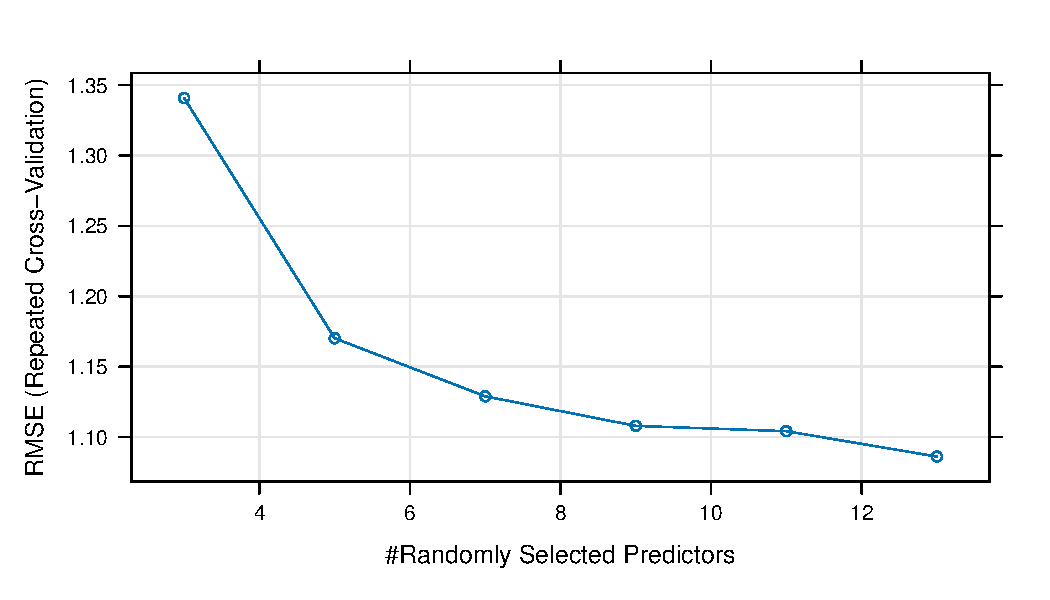
\includegraphics{Modelling_Energy_Intensity-V3_files/figure-pdf/rf-tune-1.pdf}

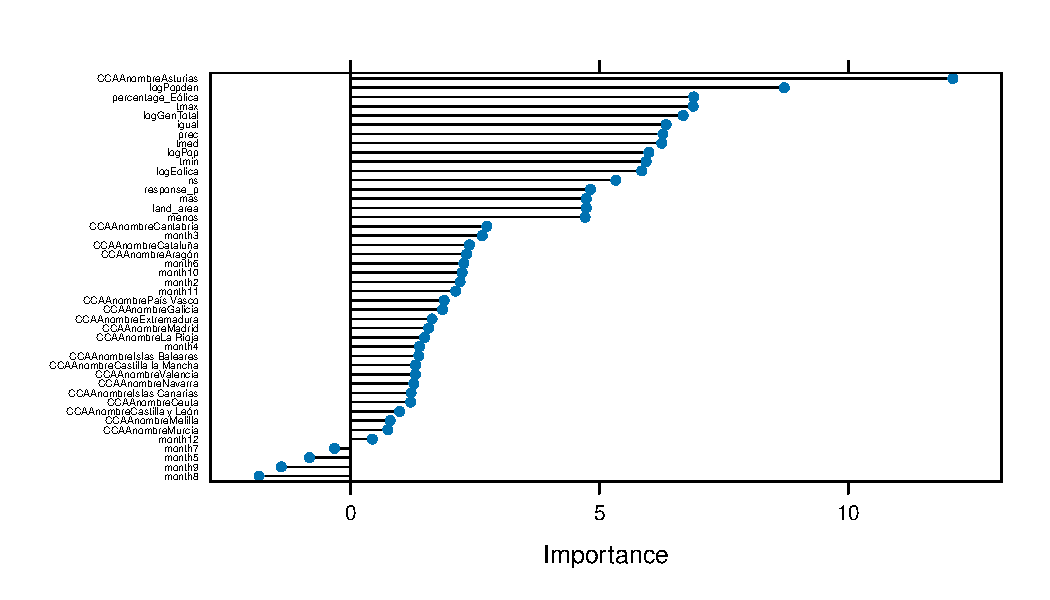
\includegraphics{Modelling_Energy_Intensity-V3_files/figure-pdf/unnamed-chunk-3-1.pdf}

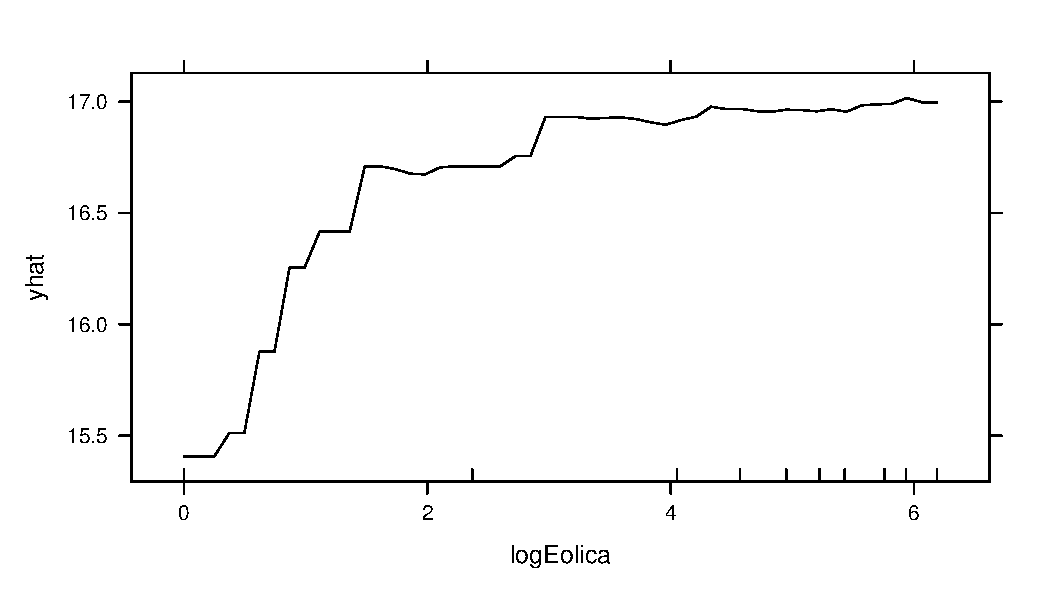
\includegraphics{Modelling_Energy_Intensity-V3_files/figure-pdf/unnamed-chunk-3-2.pdf}

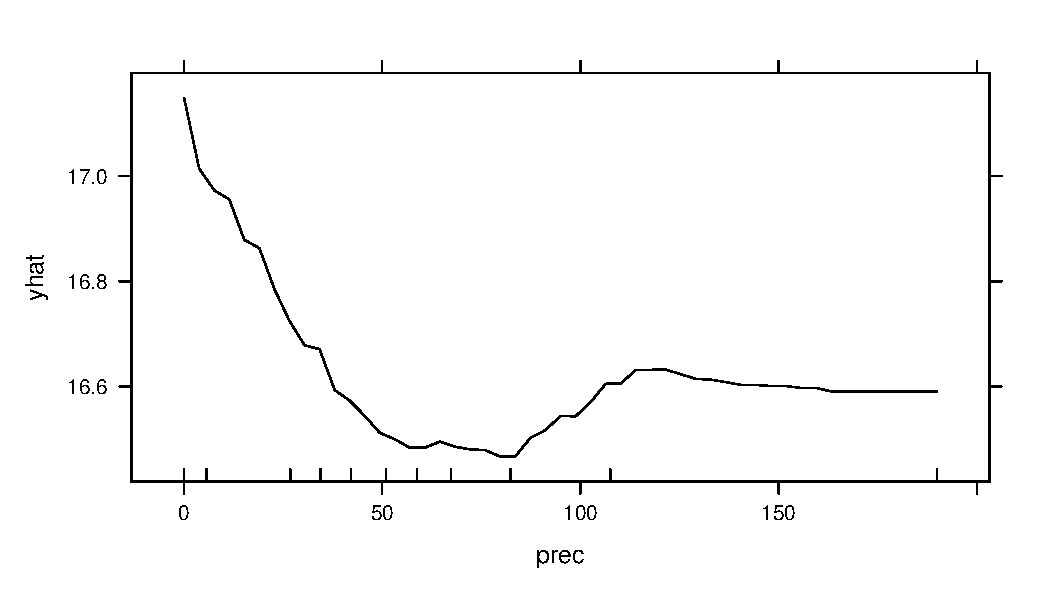
\includegraphics{Modelling_Energy_Intensity-V3_files/figure-pdf/unnamed-chunk-3-3.pdf}

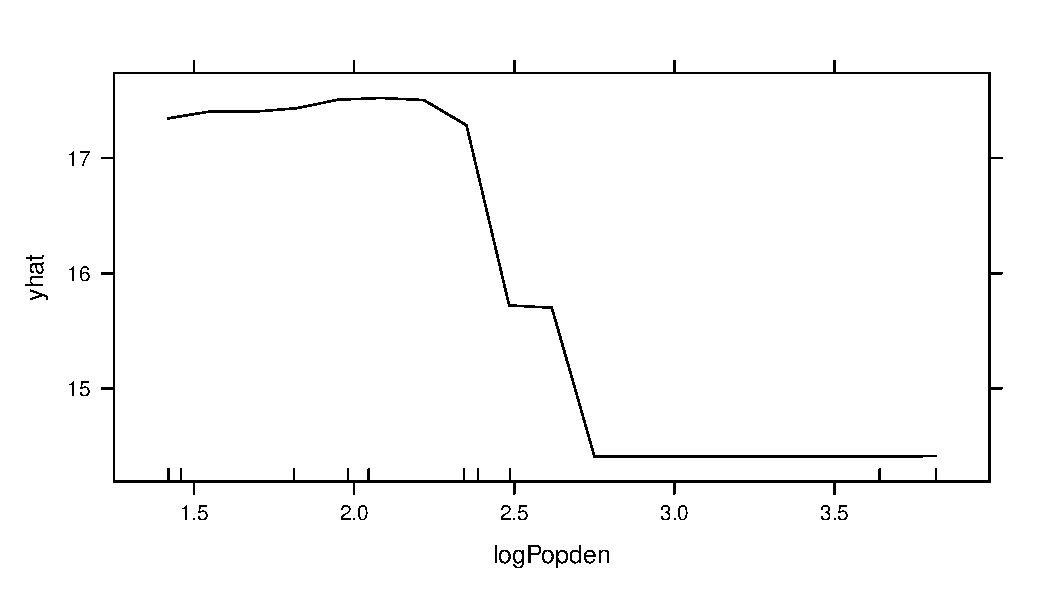
\includegraphics{Modelling_Energy_Intensity-V3_files/figure-pdf/unnamed-chunk-3-4.pdf}

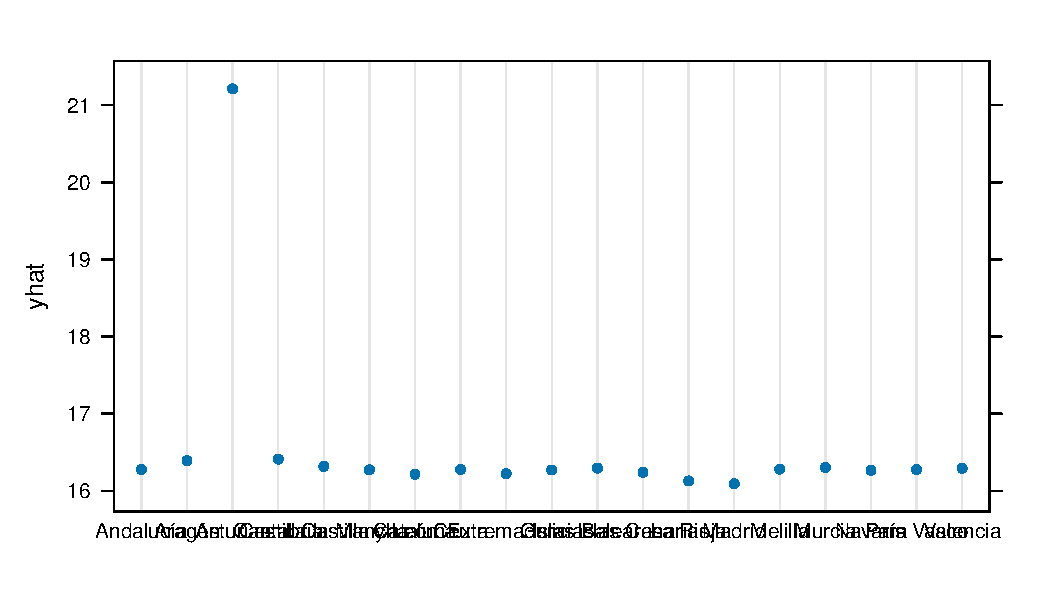
\includegraphics{Modelling_Energy_Intensity-V3_files/figure-pdf/unnamed-chunk-3-5.pdf}

According to random forest, which gets really good R\textsuperscript{2}
and RMSE when testing against 2014 data, the month variable is not
important. Most important is whether or not the CCAA is
\textbf{Asturias}. Then the next top predictors are survey results,
electricity generated and population density.

\hypertarget{rf-without-ccaa}{%
\section{RF without CCAA}\label{rf-without-ccaa}}

I decided to run a \emph{Random Forest} model without a variable for
CCAA. This removal should show us which variables are important to
predict energy intensity, without directly asking, ``Which autonomous
community is this?'' Although one possibility would be only keep the
binary dummy variable for when CCAA is equal to Asturias.

I also removed \texttt{month} because it has not shown to be important
without CCAA involved.

This shrunken model with fewer explanatory variables had somewhat
similar results. The most important variable was if the CCAA was
Asturias. That was such a big outlier I had to keep it as a binary
variable. The other most important variables were average temperature
and the survey results for \texttt{igual}.

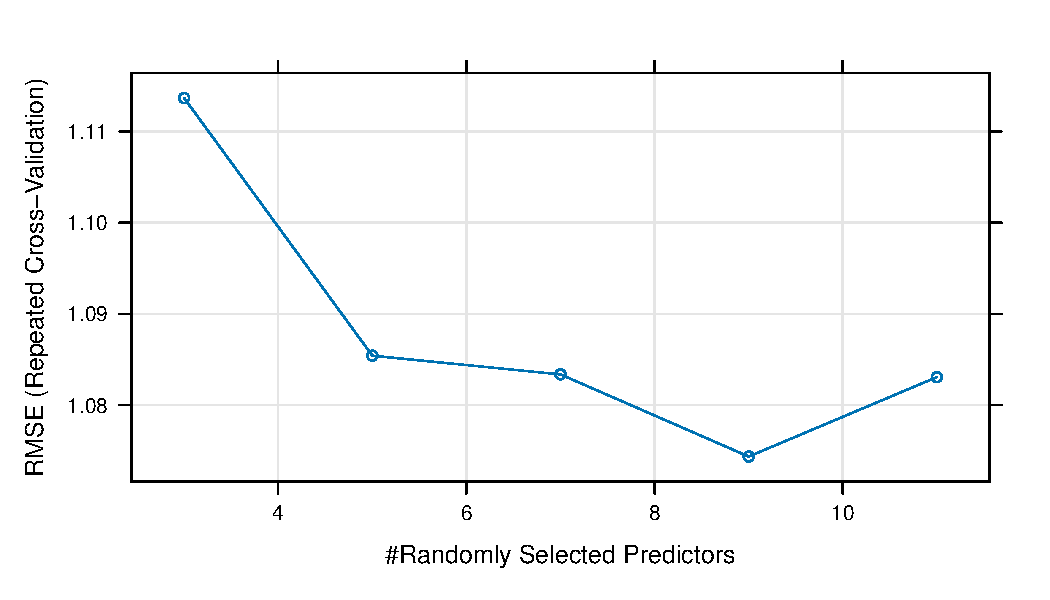
\includegraphics{Modelling_Energy_Intensity-V3_files/figure-pdf/unnamed-chunk-5-1.pdf}

\begin{figure}

{\centering 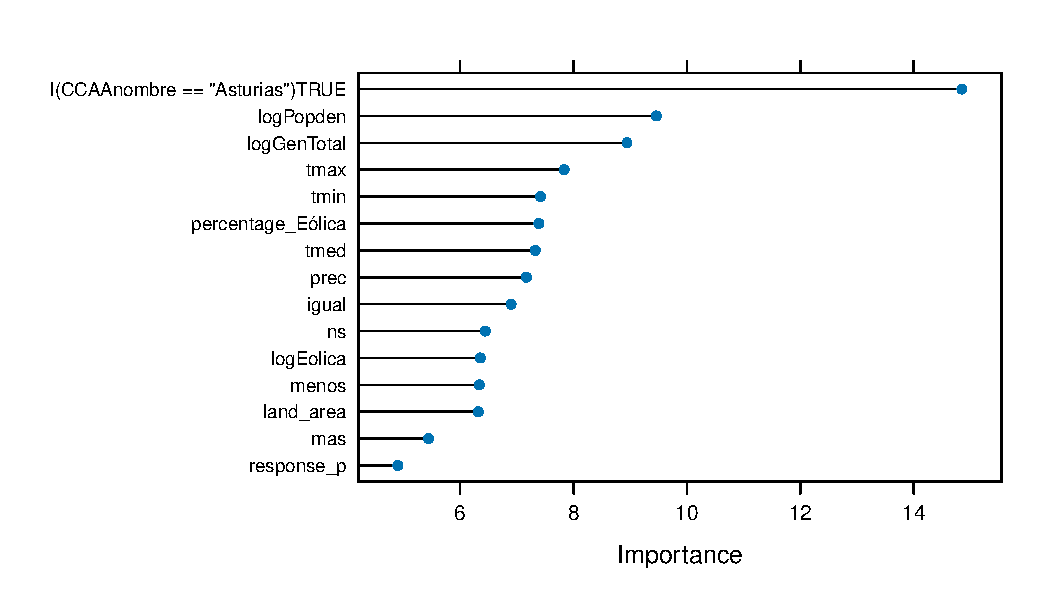
\includegraphics{Modelling_Energy_Intensity-V3_files/figure-pdf/unnamed-chunk-6-1.pdf}

}

\caption{Random forest without CCAA and Month}

\end{figure}

\begin{figure}

{\centering 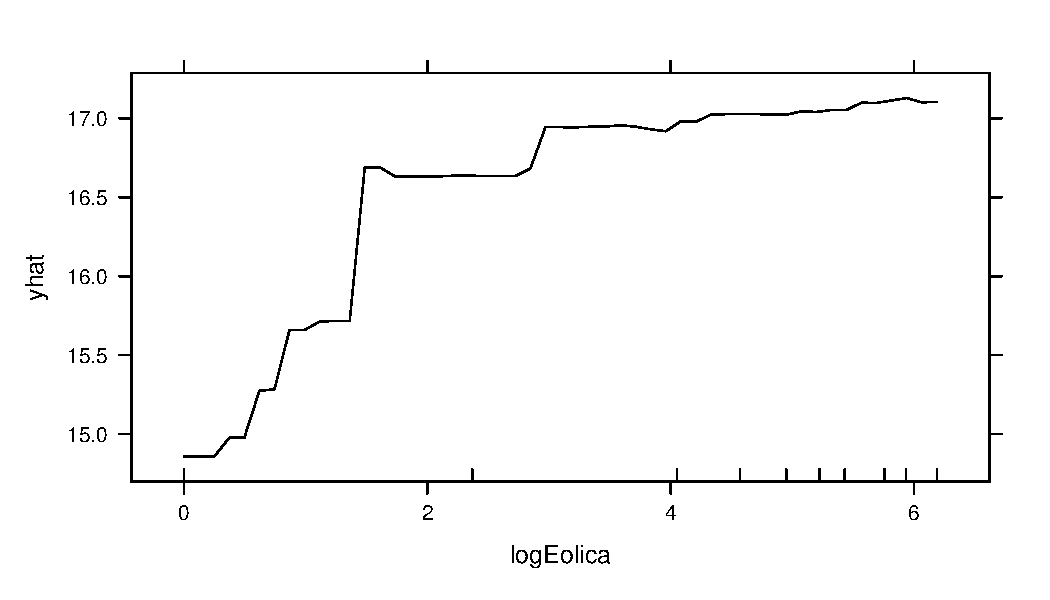
\includegraphics{Modelling_Energy_Intensity-V3_files/figure-pdf/unnamed-chunk-6-2.pdf}

}

\caption{Random forest without CCAA and Month}

\end{figure}

\begin{figure}

{\centering 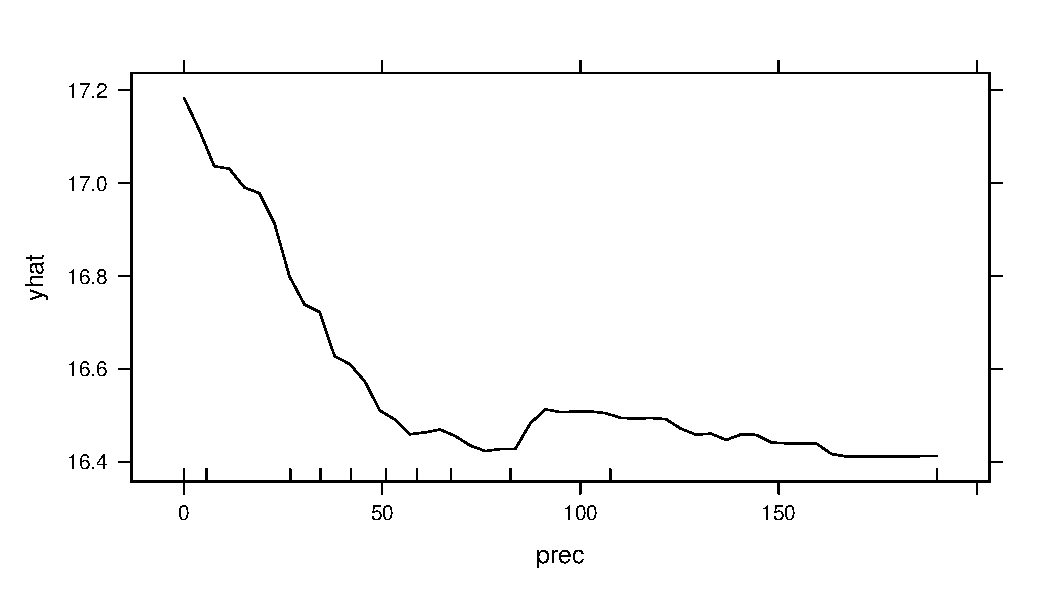
\includegraphics{Modelling_Energy_Intensity-V3_files/figure-pdf/unnamed-chunk-6-3.pdf}

}

\caption{Random forest without CCAA and Month}

\end{figure}

\begin{figure}

{\centering 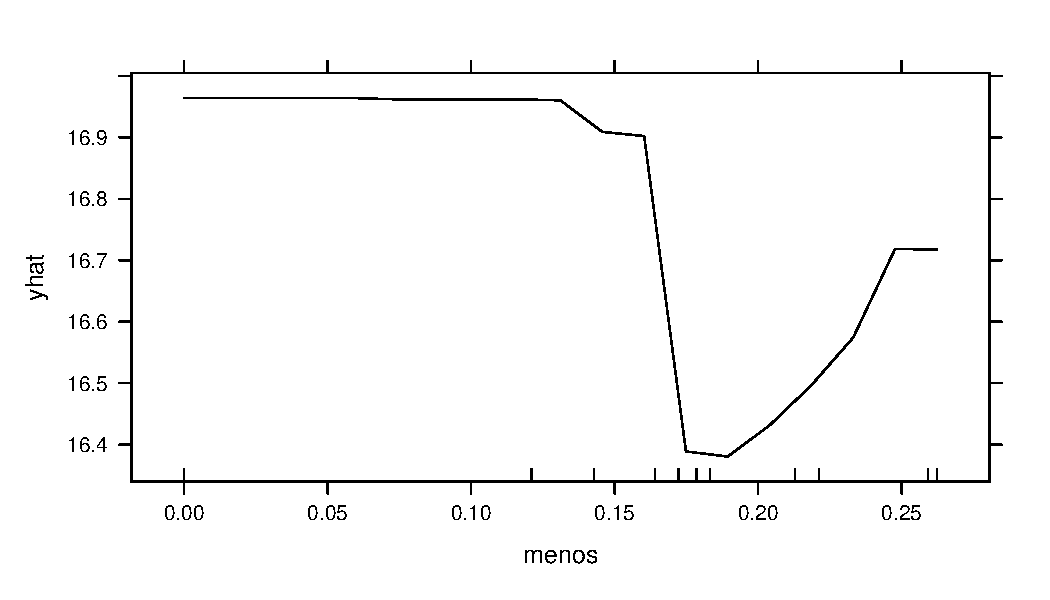
\includegraphics{Modelling_Energy_Intensity-V3_files/figure-pdf/unnamed-chunk-6-4.pdf}

}

\caption{Random forest without CCAA and Month}

\end{figure}

\begin{figure}

{\centering 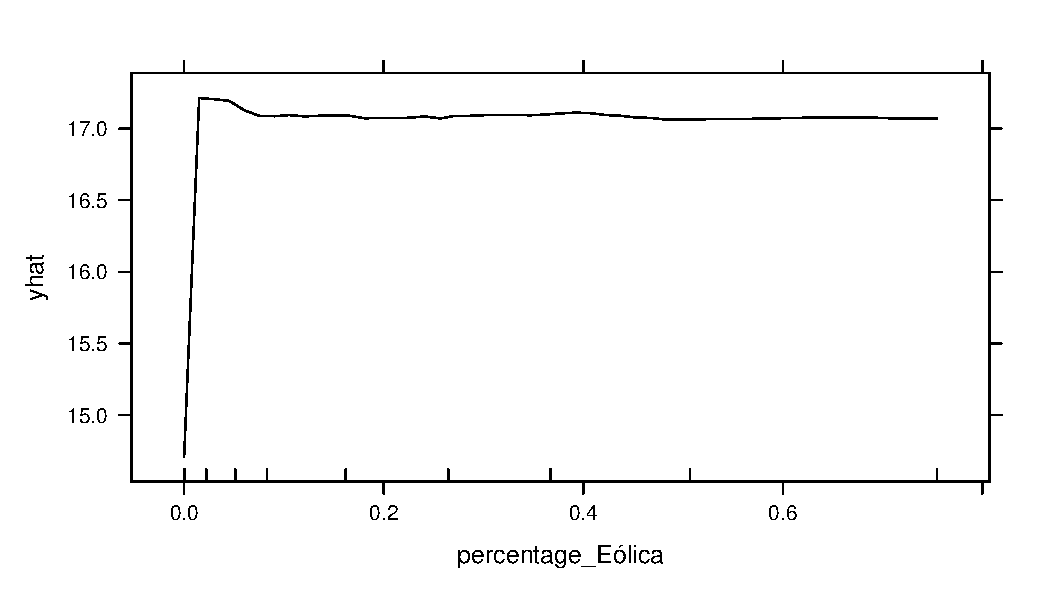
\includegraphics{Modelling_Energy_Intensity-V3_files/figure-pdf/unnamed-chunk-6-5.pdf}

}

\caption{Random forest without CCAA and Month}

\end{figure}

\begin{verbatim}
[1] "random forest w/out CCAA stats:"
\end{verbatim}

\begin{verbatim}
     RMSE  Rsquared       MAE 
6.7381884 0.8204256 5.8364620 
\end{verbatim}

\hypertarget{rf-with-small-list-of-variables}{%
\section{RF with small list of
variables}\label{rf-with-small-list-of-variables}}

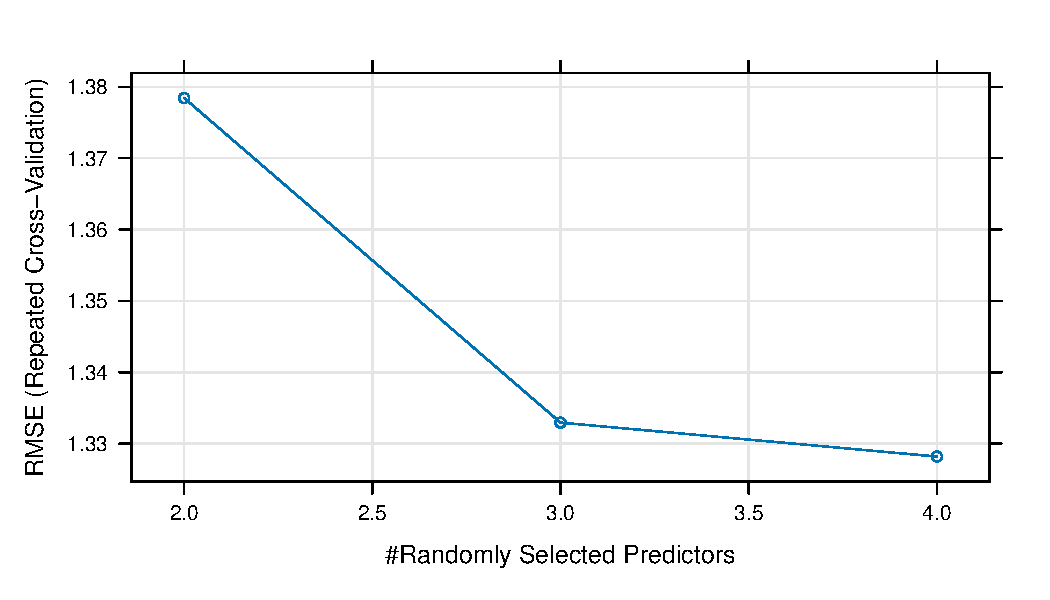
\includegraphics{Modelling_Energy_Intensity-V3_files/figure-pdf/unnamed-chunk-8-1.pdf}

\begin{figure}

{\centering 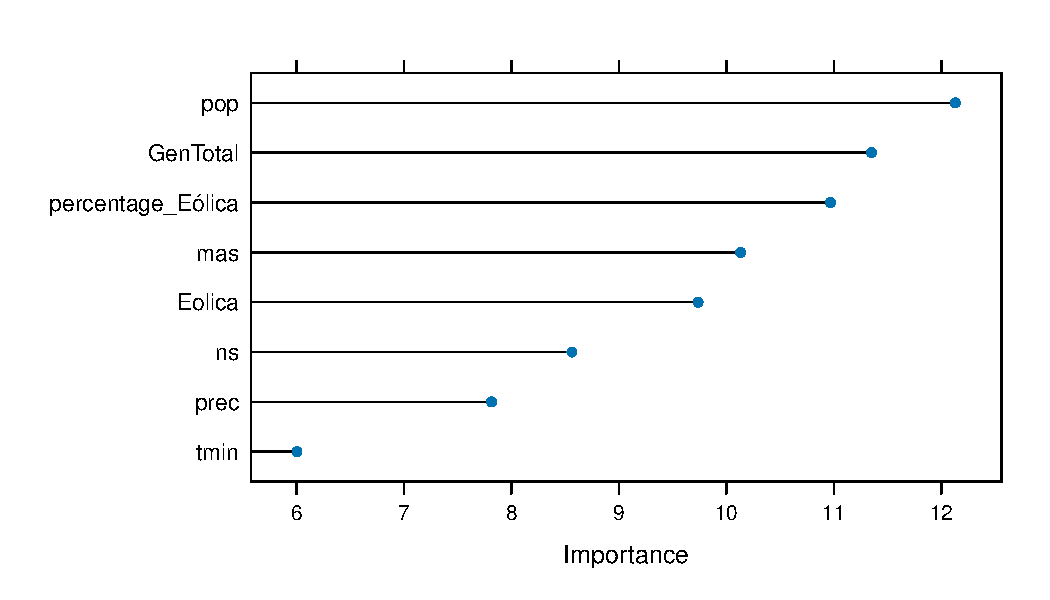
\includegraphics{Modelling_Energy_Intensity-V3_files/figure-pdf/unnamed-chunk-9-1.pdf}

}

\caption{Random forest with small list of variables}

\end{figure}

\begin{figure}

{\centering 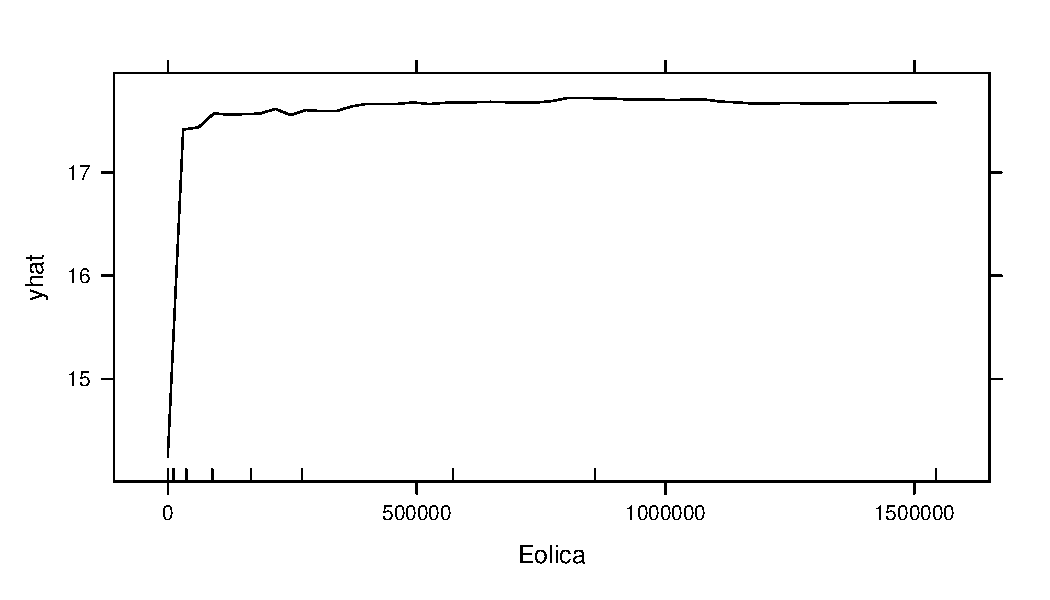
\includegraphics{Modelling_Energy_Intensity-V3_files/figure-pdf/unnamed-chunk-9-2.pdf}

}

\caption{Random forest with small list of variables}

\end{figure}

\begin{figure}

{\centering 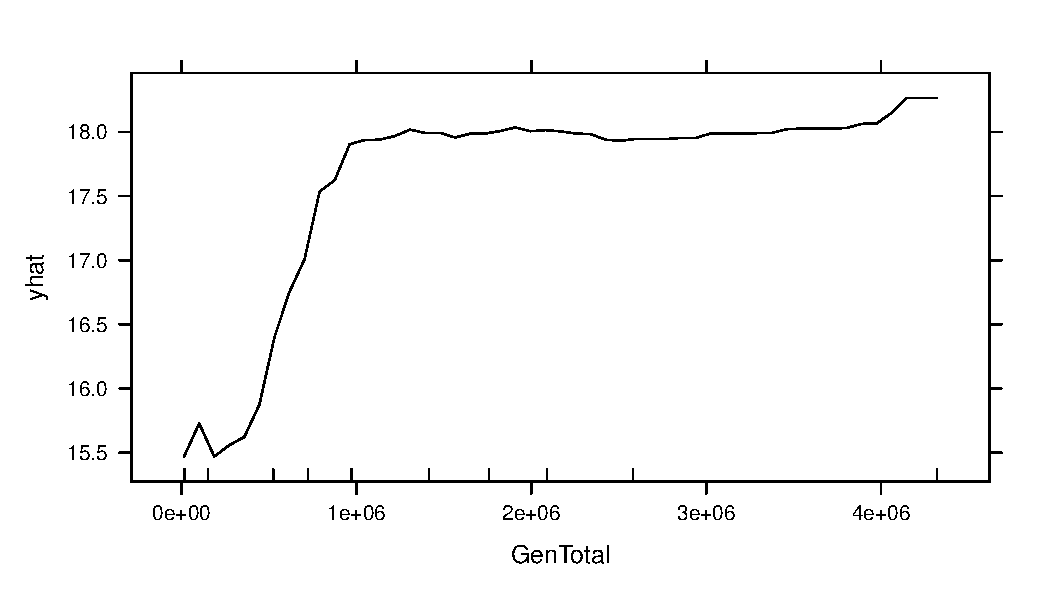
\includegraphics{Modelling_Energy_Intensity-V3_files/figure-pdf/unnamed-chunk-9-3.pdf}

}

\caption{Random forest with small list of variables}

\end{figure}

\begin{figure}

{\centering 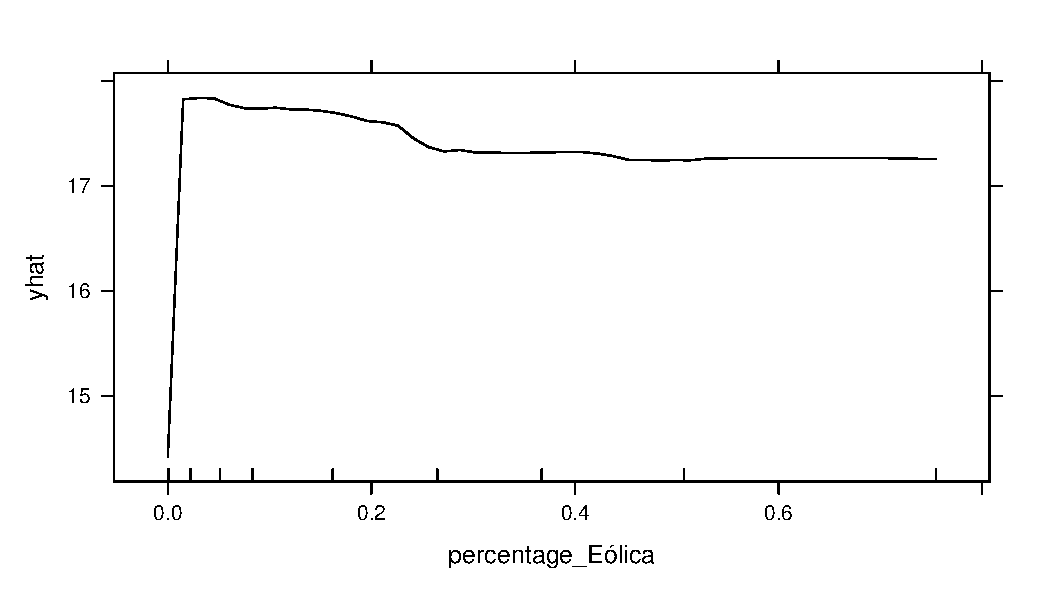
\includegraphics{Modelling_Energy_Intensity-V3_files/figure-pdf/unnamed-chunk-9-4.pdf}

}

\caption{Random forest with small list of variables}

\end{figure}

\begin{figure}

{\centering 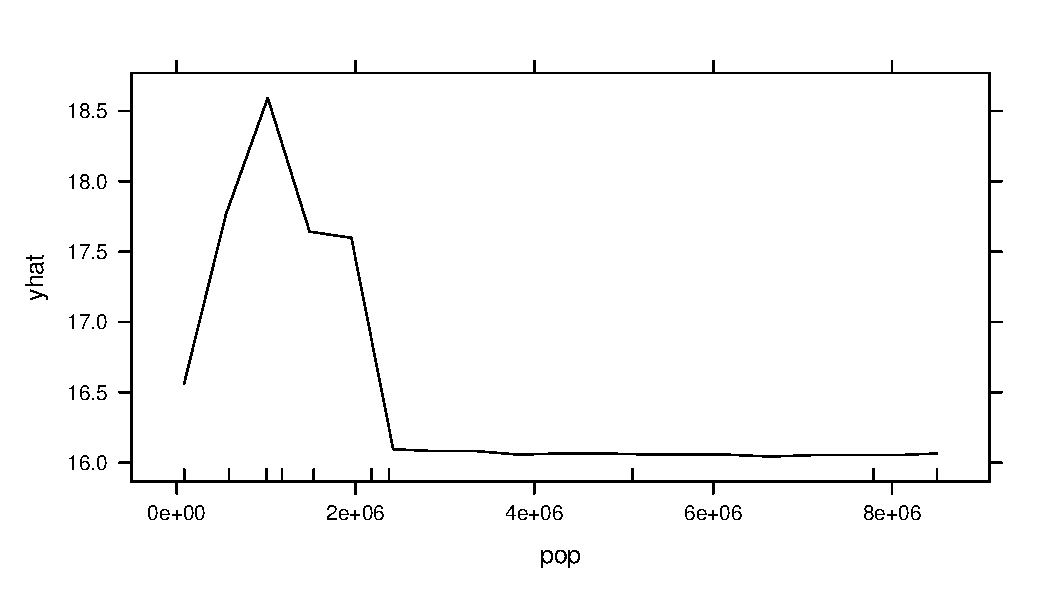
\includegraphics{Modelling_Energy_Intensity-V3_files/figure-pdf/unnamed-chunk-9-5.pdf}

}

\caption{Random forest with small list of variables}

\end{figure}

\begin{verbatim}
[1] "random forest w/small list of vars:"
\end{verbatim}

\begin{verbatim}
     RMSE  Rsquared       MAE 
7.4193017 0.7779909 6.2560649 
\end{verbatim}

\hypertarget{regularized-regression}{%
\section{Regularized regression}\label{regularized-regression}}

\textbf{ElasticNet with CCAA :}

Regularized regression methods are good for reducing the strength of
explanatory variables that are highly correlated with other variables.
Many explanatory variables in the model are collinear, like the cliamte
data and the survey data.

Based off what we know from the previous analyzes, we can predict that
CCAA will be a very important variable, even if it is used to detect
\textbf{Asturias}.

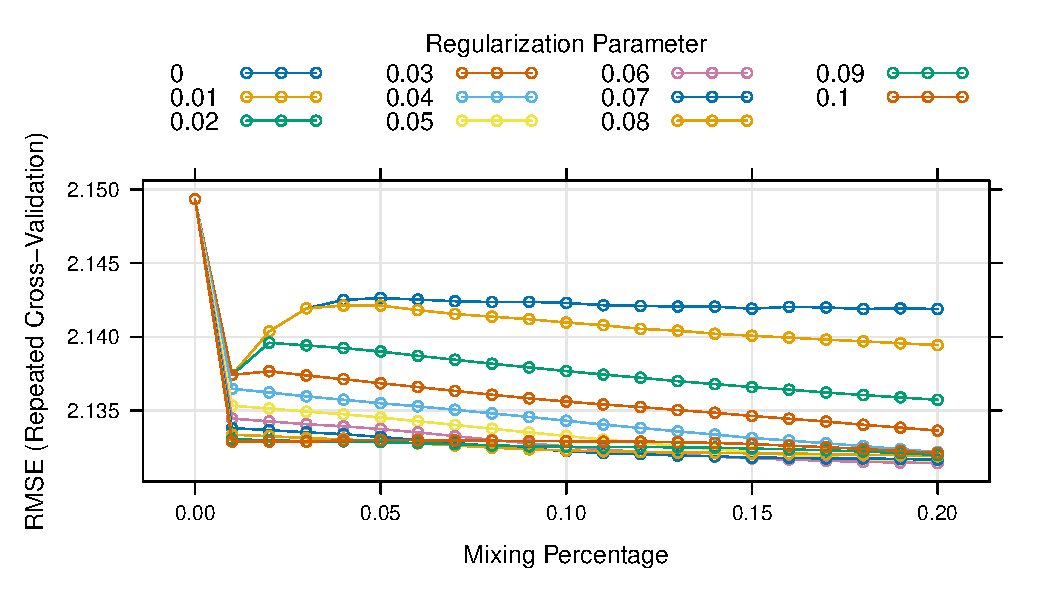
\includegraphics{Modelling_Energy_Intensity-V3_files/figure-pdf/glmnet_test-1.pdf}

\begin{verbatim}
    alpha lambda
227   0.2   0.06
\end{verbatim}

\begin{verbatim}
     RMSE  Rsquared       MAE 
6.9267423 0.8151508 5.8209213 
\end{verbatim}

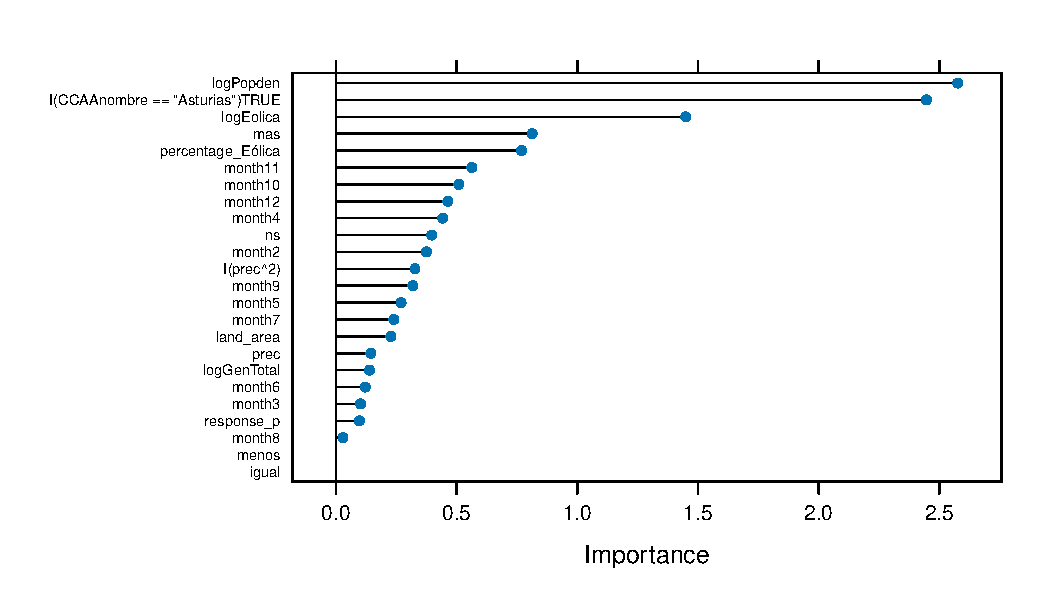
\includegraphics{Modelling_Energy_Intensity-V3_files/figure-pdf/unnamed-chunk-11-1.pdf}

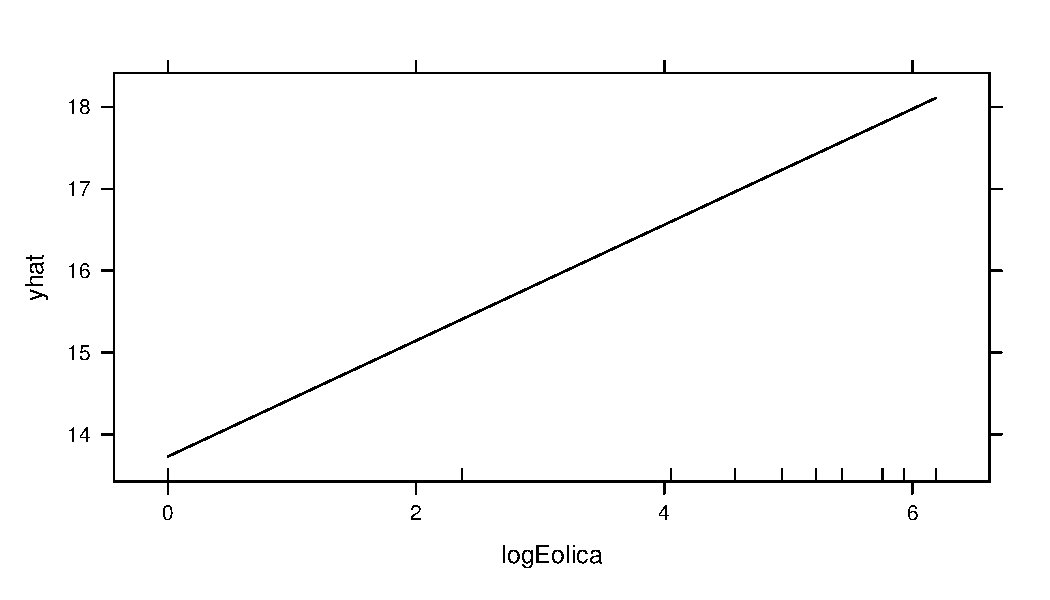
\includegraphics{Modelling_Energy_Intensity-V3_files/figure-pdf/unnamed-chunk-11-2.pdf}

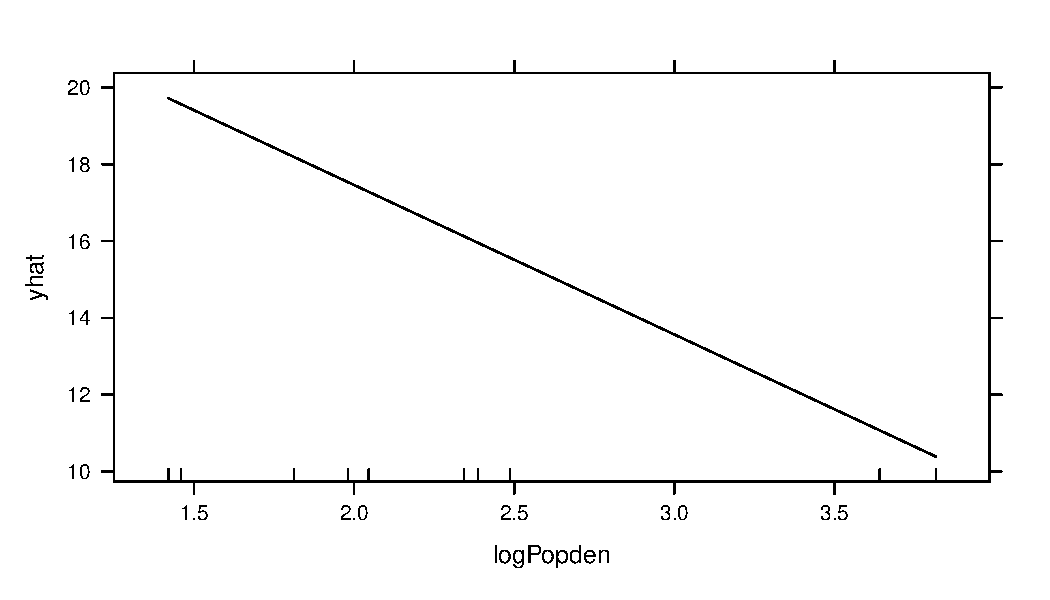
\includegraphics{Modelling_Energy_Intensity-V3_files/figure-pdf/unnamed-chunk-11-3.pdf}

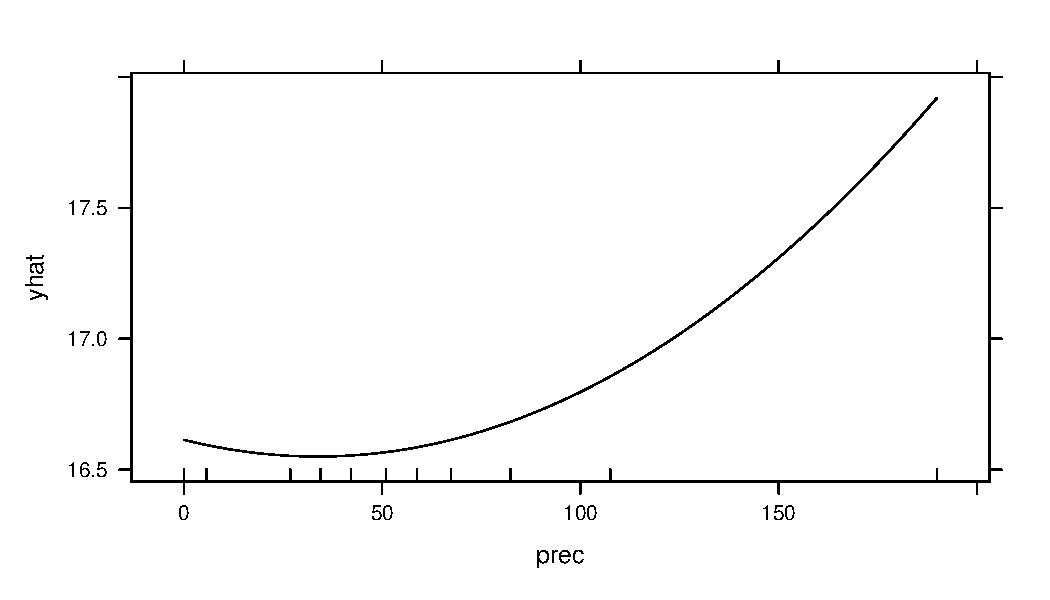
\includegraphics{Modelling_Energy_Intensity-V3_files/figure-pdf/unnamed-chunk-11-4.pdf}

The elastic net model does a lot better than the other linear models
based off R\textsuperscript{2}.

\textbf{ElasticNet: without CCAA}

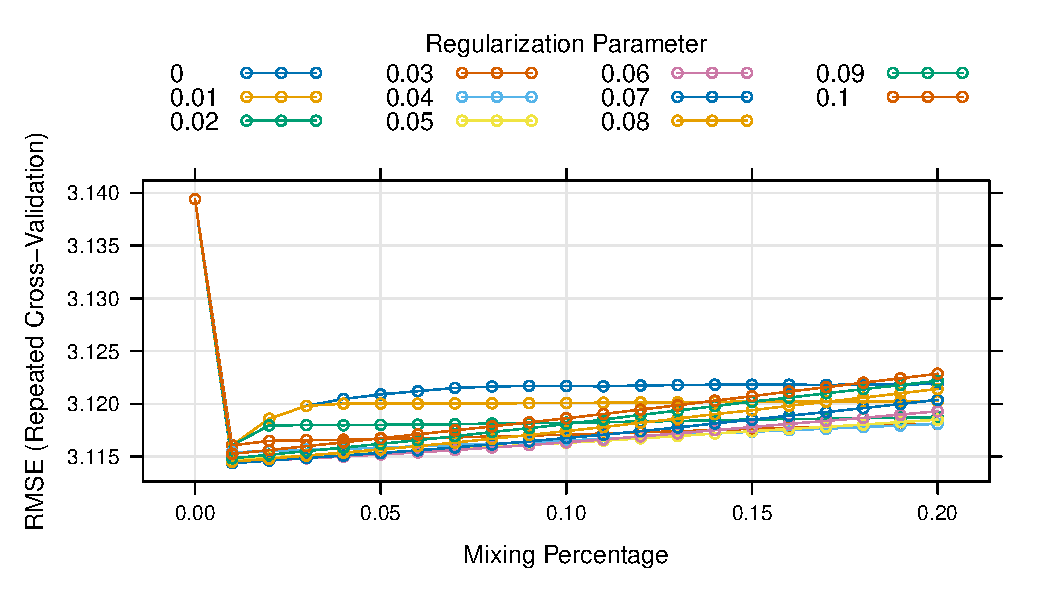
\includegraphics{Modelling_Energy_Intensity-V3_files/figure-pdf/unnamed-chunk-12-1.pdf}

\begin{verbatim}
   alpha lambda
19  0.01   0.07
\end{verbatim}

\begin{verbatim}
     RMSE  Rsquared       MAE 
7.6747401 0.5893468 5.9757730 
\end{verbatim}

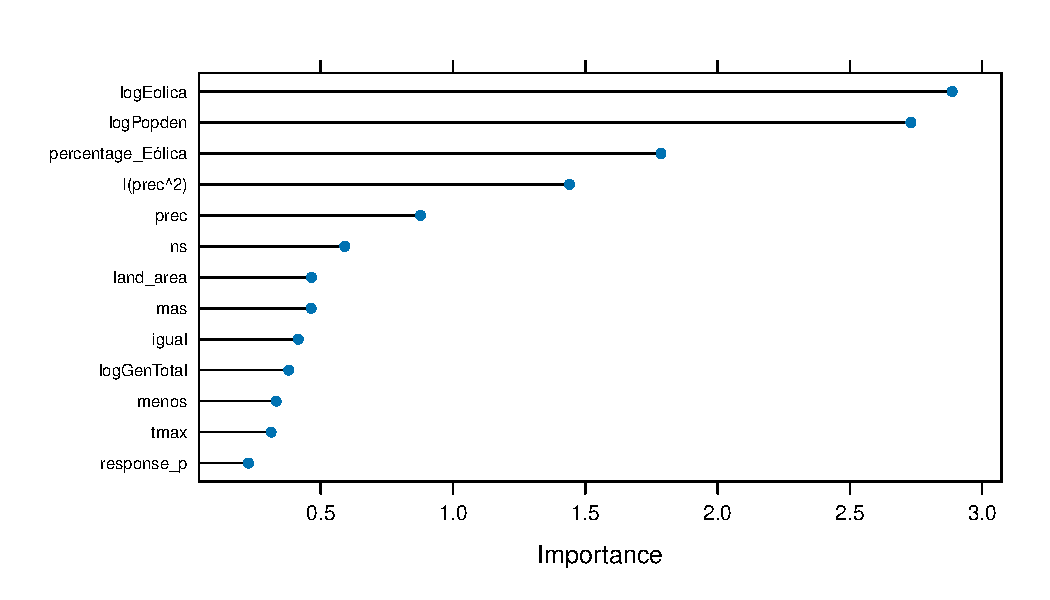
\includegraphics{Modelling_Energy_Intensity-V3_files/figure-pdf/unnamed-chunk-13-1.pdf}

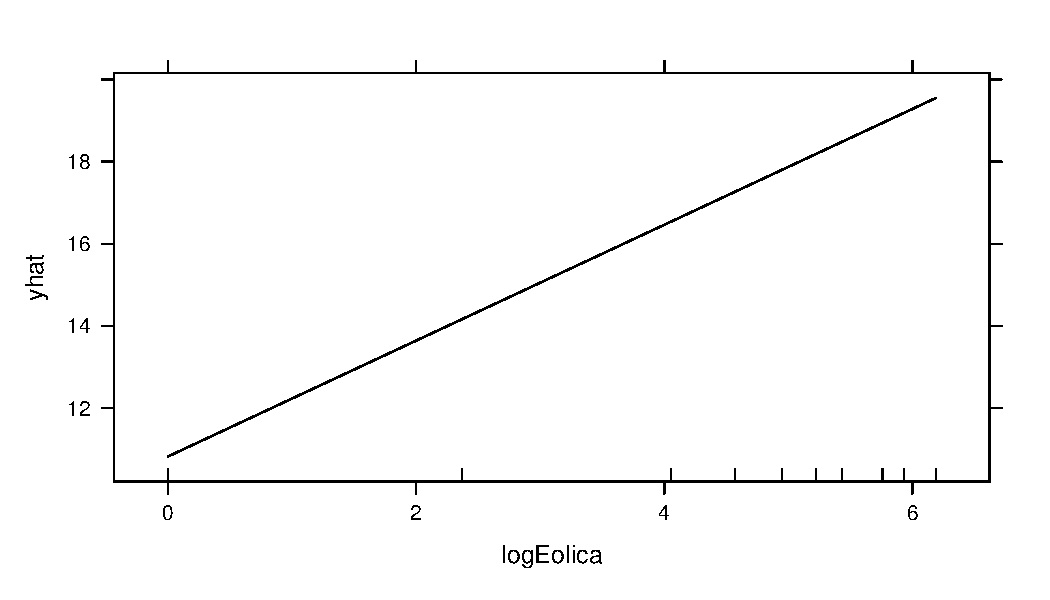
\includegraphics{Modelling_Energy_Intensity-V3_files/figure-pdf/unnamed-chunk-13-2.pdf}

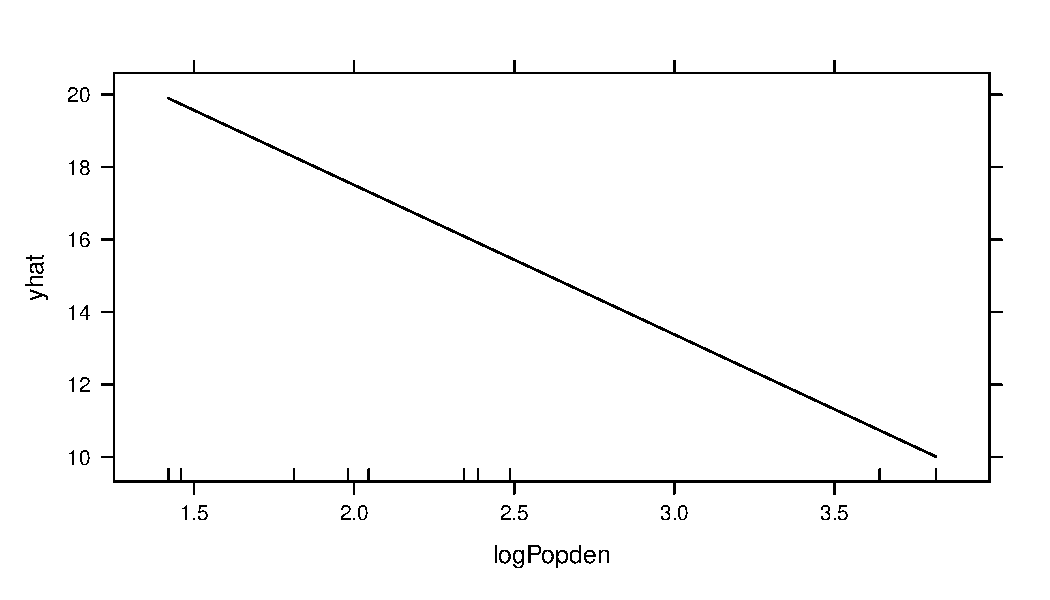
\includegraphics{Modelling_Energy_Intensity-V3_files/figure-pdf/unnamed-chunk-13-3.pdf}

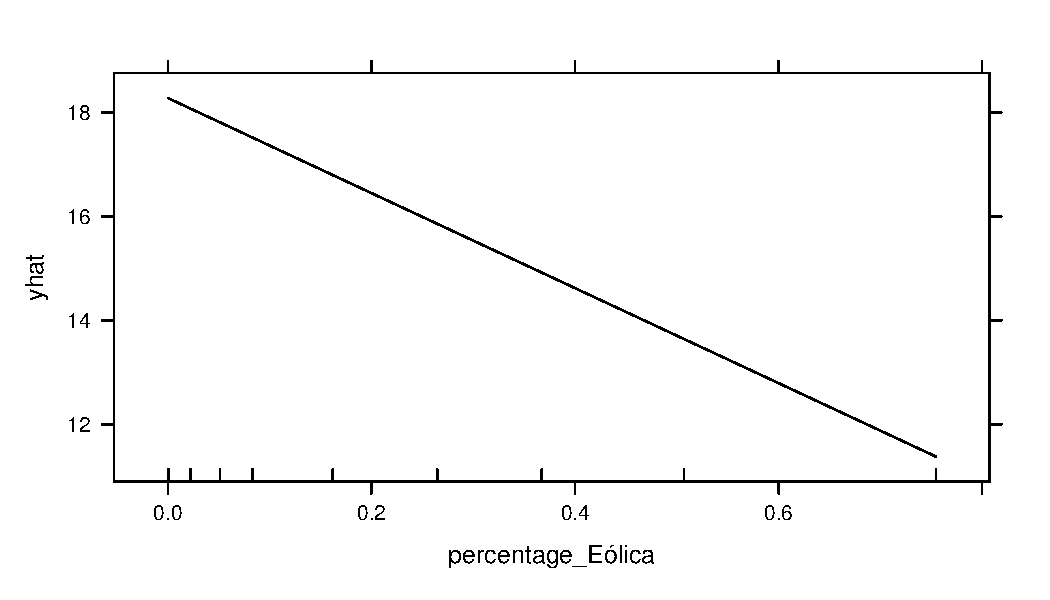
\includegraphics{Modelling_Energy_Intensity-V3_files/figure-pdf/unnamed-chunk-13-4.pdf}

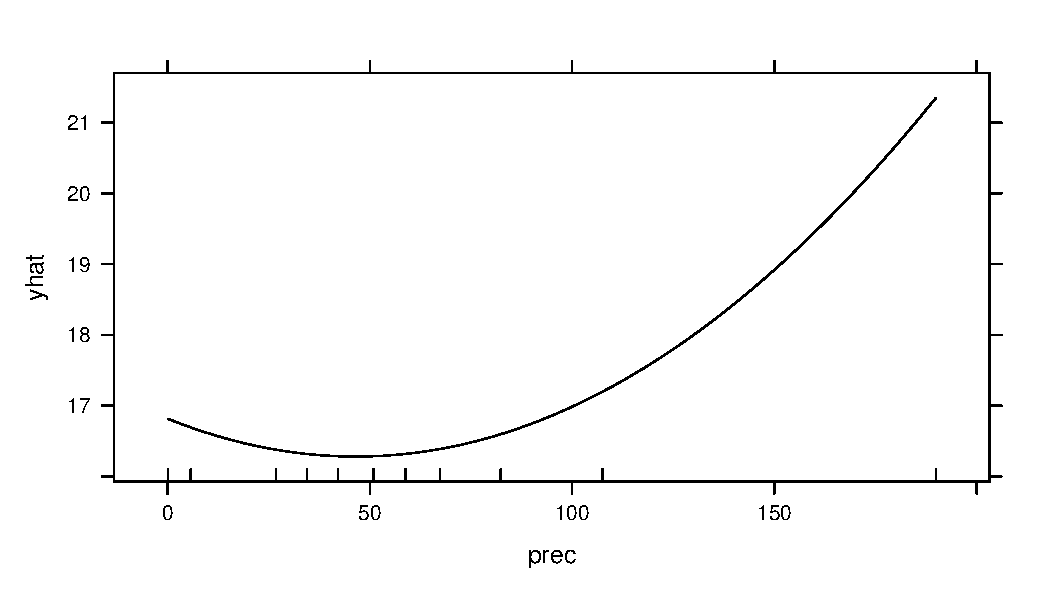
\includegraphics{Modelling_Energy_Intensity-V3_files/figure-pdf/unnamed-chunk-13-5.pdf}

\hypertarget{interpretations-without-ccaa}{%
\subsubsection{Interpretations without
CCAA}\label{interpretations-without-ccaa}}

Now we can see how much the differences between CCAA effect the energy
intensity in ways I have not already included in the data. First of all,
the R\textsuperscript{2} is a lot lower, but that is expected.

\begin{itemize}
\tightlist
\item
  The most important variables now are logged population density and
  logged wind energy generated.
\item
  Land area and logged total electricity generated are considered
  somewhat important
\end{itemize}

Interesting that without the CCAA variable, the most important
predictors change. This tells me that differences across regions make a
huge difference. One important difference is climate and geography.
Other factors could include investment in modern technology.

\hypertarget{comparing-test-results}{%
\section{Comparing test results}\label{comparing-test-results}}

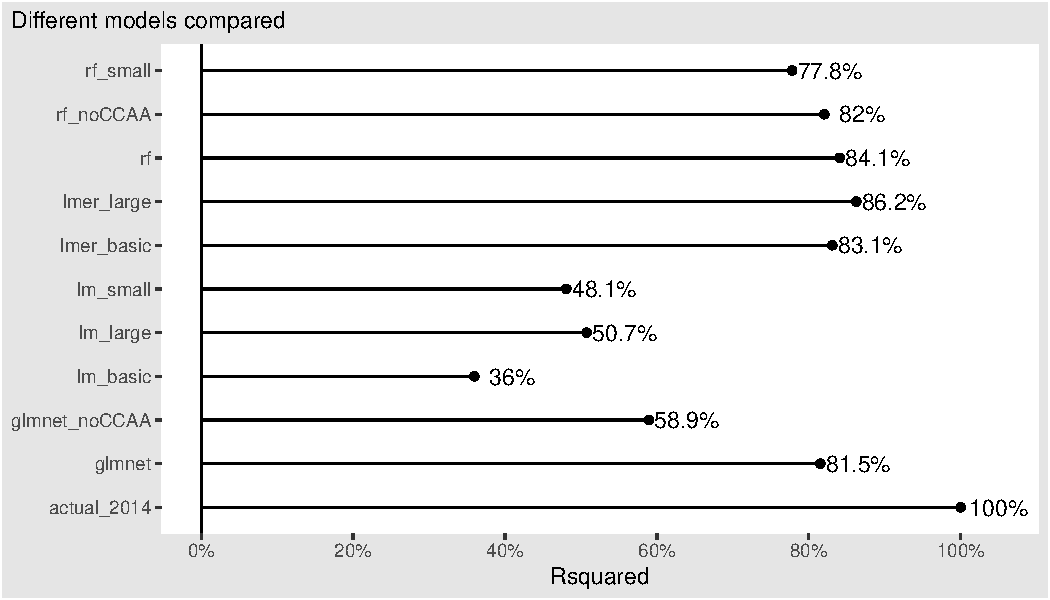
\includegraphics{Modelling_Energy_Intensity-V3_files/figure-pdf/unnamed-chunk-15-1.pdf}

The ordinary linear regression models perform the worst. They are worse
than the RF without CCAA. I think this is because RF uses non-linear
techniques of manipulating the predictors and find the results in ways
that linear regression cannot. Also, removing CCAA from the equation has
a big factor in linear techniques.

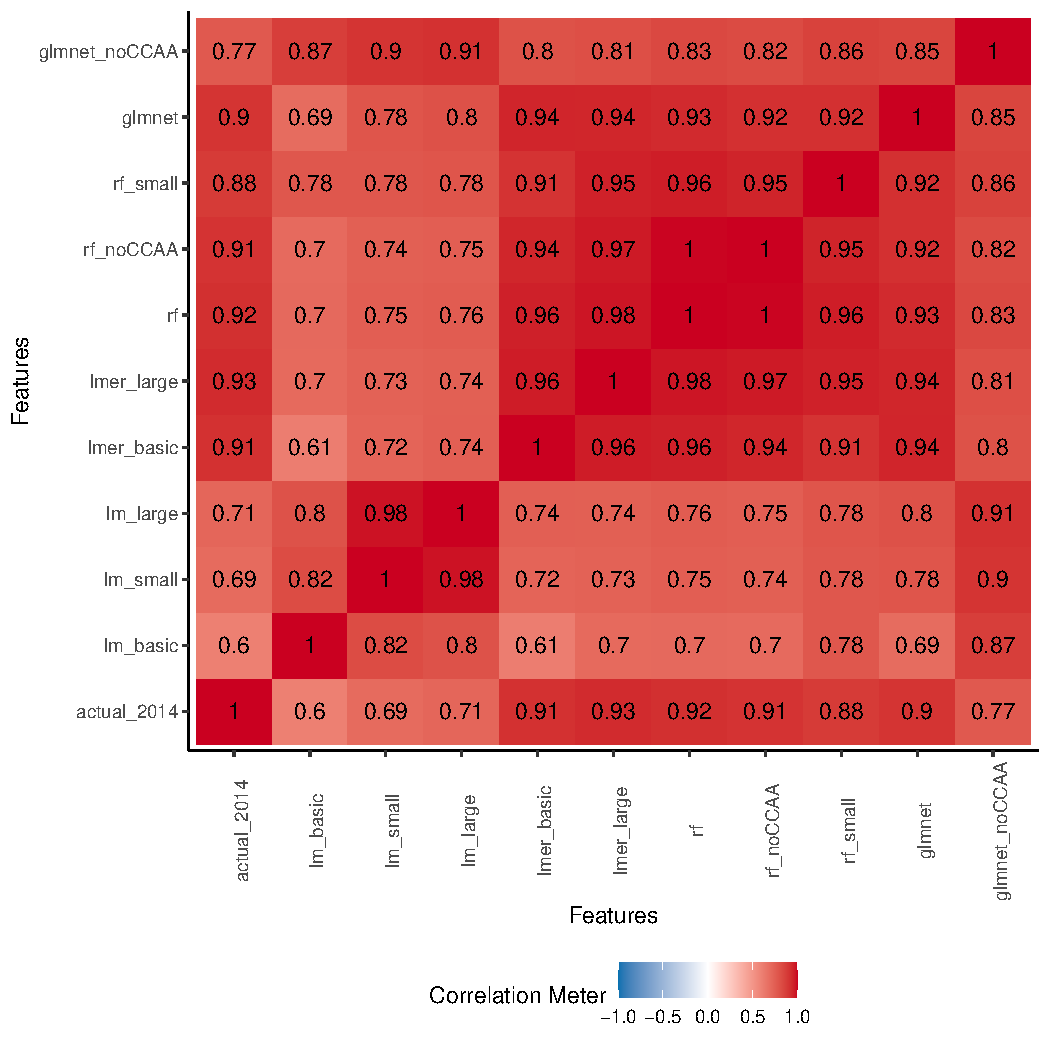
\includegraphics{Modelling_Energy_Intensity-V3_files/figure-pdf/unnamed-chunk-16-1.pdf}

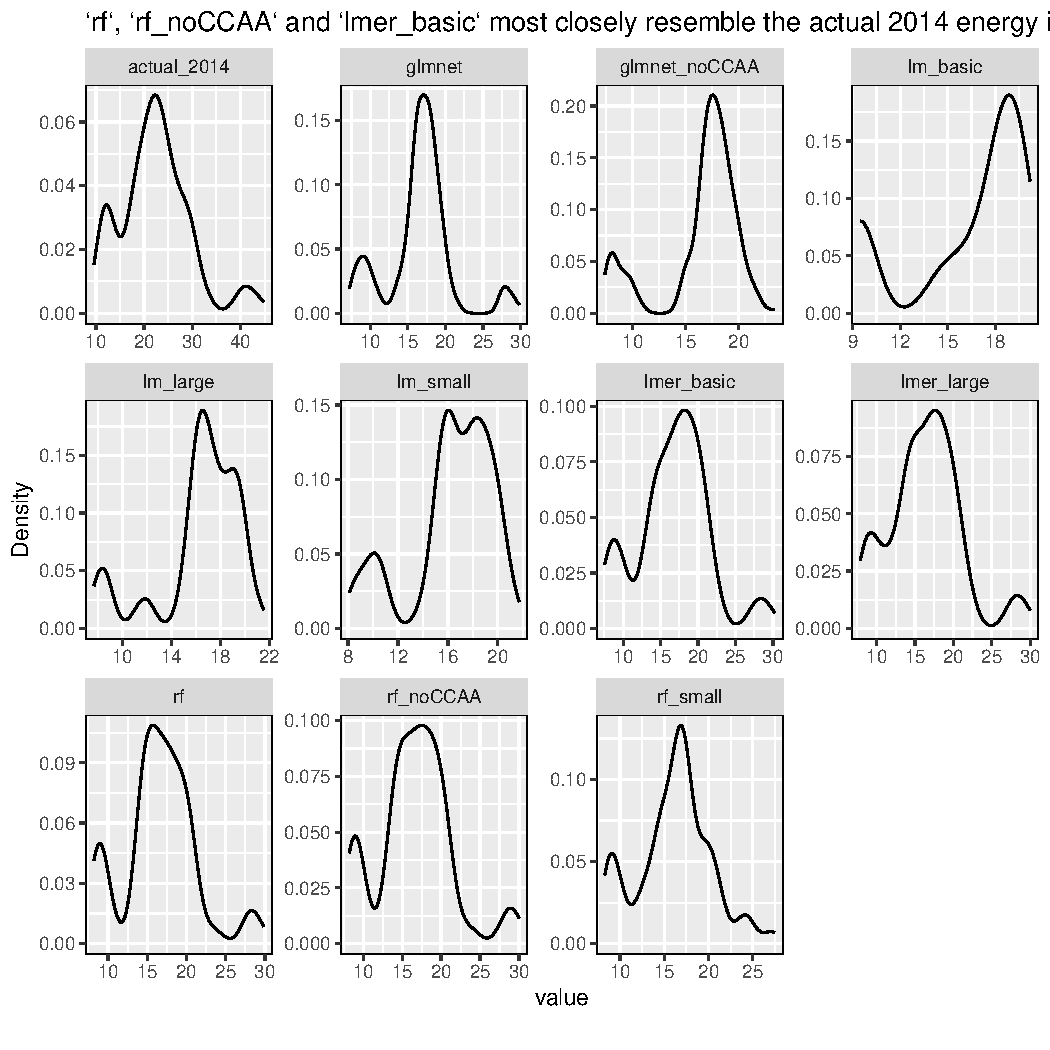
\includegraphics{Modelling_Energy_Intensity-V3_files/figure-pdf/unnamed-chunk-16-2.pdf}



\end{document}
